% !TEX root = ../proj_report_outline.tex
\chapter{Tensor Train}\label{A:tt}

The \emph{tensor-train} (TT) decomposition has a short history -- it was first proposed in
2011 as a simpler way of representing an earlier hierarchical form derived from a
generalisation of the singular value decomposition. \autocite{Osedelets2011} It is proposed
as an alternative to the CP-decomposition as it is often easier to find a TT representation
of a given tensor.
%In the three-way case it is nearly equivalent to the more venerable Tucker 
%decomposition. \autocite{Tucker1966} The tensor train turns out to be simpler -- beyond showing the
%similarity, we consider solely the tensor-train.

The tensor-train can also be used more creatively. 
Novikov et al. \autocite{Novikov} use the decomposition to compress the final layers of a 
large convolutional neural
network by reshaping the matrices into high dimensional tensors. The reduction in parameters for
the tensor-train is most notable with particularly high-dimensional tensors, so this approach allows
for significant compression (compressing one layer up to \(200,000\) times).
They also show methods of computing the required matrix vector products
without having to expand the tensor. While this approach is highly successful, the implementation
(especially of back-propagation) is somewhat involved and it admits a very large number of ways of
applying the decomposition. To keep our search space of decompositions feasible, we consider only
the straight-forward application of the tensor-train.

\section{Description}
The tensor-train decomposition (TT-decomposition) of a general tensor \(\tensor{X}\) with
\(d\) indices is the tensor \(\tensor{Y} \approx\tensor{X}\) with elements expressed as a
product of slices of three-way tensors (so a product of matrices):
\begin{equation}
			\label{eq:tensortrain_full}
	{Y}_{i_1i_2\dots i_d} 
		= \mat{G}[1]_{\midbullet i_1 \midbullet}\mat{G}[2]_{\midbullet i_2 \midbullet}
			\cdots \mat{G}[d]_{\midbullet i_d \midbullet}.
\end{equation}
If dimension \(j\) is of size \(n_j\), then \(\tensor{G}[j]\) is size 
\(r_{j-1} \times n_j \times r_{j}\) so that each slice \(\mat{G}[j]_{\midbullet i \midbullet}\)
is size \(r_{j-1} \times r_{j}\). The collection of \(r_i\) is the `tt-rank' of the
decomposition and controls the number of parameters. In order to ensure the result of the chain
of matrix products is a scalar, it must be that \(r_0 = r_d = 1\). \autocite{Osedelets2011}

The three-way case presents no obvious simplifications from the general case but we present it
here to ensure consistent notation through the remainder of this section. The TT-decomposition
of a three-way tensor of size \(n_1 \times n_2 \times n_3\) has three `cores' with shapes
\(1 \times n_1 \times r_1\), \(r_1 \times n_2 \times r_2\) and \(r_2 \times n_3 \times 1\). For
convenience, we can treat these as a matrix, a three-way tensor and a matrix by ignoring 
dimensions of size one. This leads to the following expression of 
equation~\ref{eq:tensortrain_full} where \(\tensor{W}\) is the three way tensor in its
decomposed form:
\begin{equation} \label{eq:tensortrain_three}
	W_{ijk} = \mat{A}_{i\midbullet} \mat{B}_{\midbullet j \midbullet} \mat{C}_{\midbullet k}.
\end{equation} In a manner consistent with the CP-decomposition we denote such a decomposed
tensor \(\tensor{W} = [\mat{A},\tensor{B},\mat{C}]_{TT}\). It is important to note that the
shapes are less consistent: \(\mat{A}\) is an \(n_1 \times r_1\) matrix, \(\tensor{B}\) a
\(r_1 \times n_2 \times r_1\) tensor and \(\mat{C}\) an \(r_2 \times n_3\) matrix.

As this decomposition only contains contractive products, it is very well expressed as a Tensor
Network diagram. Figure~\ref{fig:tttnds} shows both the general case and the three-way case --
the general case shows clearly how we can build a tensor with a large number of dimensions purely
out of relatively small three-way tensors. 
%The Tucker decomposition is also presented to illustrate
%the similarities in the three-way case. It is also worth contrasting with figure~\ref{fig:cpbilintnd}
%to see how the CP-decomposition can arise as a special case, a notion which is formalised later.

\begin{figure}
	\centering
	\begin{subfigure}[t]{0.45\textwidth}
		\begin{tikzpicture}
		\draw
				(2,0) -- (1,0) node[label=below:{\(\mat{A}\)}]{}
				-- (0,0)
				(-2,0) -- (-1,0) node[label=below:{\(\mat{C}\)}]{}
				-- (0,0)
				(0,0) node[label=below:{\(\tensor{B}\)}]{} -- (0,1)
			;
		\end{tikzpicture}
		\caption{Three-way tensor train.}
	\end{subfigure}~
%	\begin{subfigure}[t]{0.45\textwidth}
%		\begin{tikzpicture}
%		\draw
%				(2,0) -- (1,0) node[label=below:{\(\mat{C}\)}]{}
%				-- (0,0)
%				(-2,0) -- (-1,0) node[label=below:{\(\mat{A}\)}]{}
%				-- (0,0)
%				(0,0) node[label=below:{\(\tensor{B}\)}]{} -- (0,1)
%				-- (0,1) node[label=right:{\(\mat{C}\)}]{} -- (0,2)
%			;
%		\end{tikzpicture}
%		\caption{Three-way Tucker decomposition.}
%		\label{fig:tuckertnd}
%	\end{subfigure}\\
	\begin{subfigure}[t]{0.45\textwidth}
		\begin{tikzpicture}
		\draw
				(-2,0) -- (-1,0) node{}
				-- (0,0) node{} -- (0,1)
				(-1,0) -- (-1, 1)
				(0,0) -- (0,1)
				(0,0) -- (1,0)
				
				(2,0) -- (3,0) node{}
				-- (4,0)
				(3,0) -- (3, 1)
			;
		\path (1,0) -- node[auto=false, draw=none, fill=none] {\ldots} (2,0);
		\end{tikzpicture}
		\caption{General Tensor Train}
	\end{subfigure}
	\caption{Diagrams of the Tensor Train decomposition.}
	\label{fig:tttnds}
\end{figure}

\section{Bilinear Product}
Computing a bilinear product between two vectors and a tensor in the TT-decomposition does not
have quite such an efficient form as the CP-decomposition. Primarily this is due to the presence
of the three-way tensor \(\tensor{B}\), which means we are still eventually computing a full
tensor product, simply with a smaller tensor. We denote the product as
\begin{equation} \label{eq:tt_bilin}
	\vec{z} = \vec{x}^\mathsf{T}\mat{A}\tensor{B}\mat{C}\vec{y}.
\end{equation} For a specific index this has the form
\begin{align} \label{eq:tt_bilin_index}
	z_j &= \tran{\vec{x}}\vec{A}\mat{B}_{\midbullet j \midbullet}\mat{C}\vec{y}
		= \sum_{i}^{n_1}\sum_{k}^{n_3}
		\sum_{\alpha_1}^{r_1}
		\sum_{\alpha_2}^{r_2}A_{i\alpha_1}B_{\alpha_1j\alpha_2}C_{\alpha_2k}x_iy_k.
\end{align}

Eq.~\eqref{eq:tt_bilin} provides a clear intuition about what the TT-decomposition is doing in 
the three-way case.
Matrices \(\mat{A}\) and \(\mat{C}\) project the inputs into a new (potentially smaller) space
where the bilinear product is carried out with \(\tensor{B}\) ensuring the result has been pushed
back to the appropriate size.

\section{Gradients}
The gradient of \(\vec{z}\) with respect to \(\mat{A}\) has entries of the form:
\begin{align}
	\frac{\partial z_j}{\partial A_{lm}} 
	    &= \sum_{k}^{n_3}
		\sum_{\alpha_2}^{r_2}B_{m j\alpha_2}C_{\alpha_2k}x_ly_k
		= x_l \cdot \left(\tran{\vec{B}_{mj\midbullet}}\mat{C}\vec{y}\right). \\
\intertext{The components of the gradient with respect to \(\mat{C}\) have a similar form:}
	\frac{\partial z_j}{\partial C_{lm}} 
		&= \sum_{i}^{n_1}
		\sum_{\alpha_1}^{r_1}A_{i\alpha_1}B_{\alpha_1jl}x_iy_m 
		= y_m \cdot \left(\tran{\vec{B}_{\midbullet jl}}\mat{A}\vec{x}\right). \\
\intertext{While the gradient of the elements of \(\tensor{B}\) behave similarly
	to the CP-decomposition:}
	\frac{\partial z_j}{\partial B_{lmn}} 
		&= \sum_{i}^{n_1}\sum_{k}^{n_3}
		A_{il}C_{nk}x_iy_k. \\
\end{align}
This is very similar to the CP-decomposition. Again the central
object -- which is in this case a three-way tensor -- has highly redundant gradients, although it
is not clear what effect this may have on learning.


\section{Comparison with CP}
It is worth comparing the Tensor Train decomposition with the CP decomposition. In the three-way
case we find they are very closely related but that the CP has some key advantages. 

\subsection{Equivalence}
One condition for the tensor-train to be equivalent to the CP-decomposition is if the central
tensor in the TT-decomposition has diagonal, square slices. Intuitively this reduces the tensor
product to a matrix product. 

\begin{prop}
The rank \(R\) CP-decomposition of a tensor \(\tensor{X} = [\mat{A},\mat{B},\mat{C}]_{CP}\) is
equivalent to a TT-decomposition \([\mat{A}', \tensor{B}', \mat{C}']_{TT}\) with both ranks
equal to \(R\) and \(\tensor{B}'_{ijk} = 0\) except where \(i=k\).
\end{prop}
\begin{proof}
Consider the slices of \(\tensor{X} \in \mathbb{R}^{n_1 \times n_2 \times n_3}\) formed by fixing the
second index and allowing the first and third to vary. If 
\(\tensor{X} = [\mat{A}, \mat{B}, \mat{C}]_{CP}\) then these slices can be expressed concisely as
\begin{equation} \label{eq:cp-slice}
	\mat{X}_{\midbullet j \midbullet} = \mat{A}\diag({\mat{B}_{j\midbullet}})\tran{\mat{C}}
\end{equation} where \(\diag(\vec{v})\) denotes the matrix with vector \(\vec{v}\) along the
leading diagonal and zero elsewhere. 
It is clear the the diagonal matrix must then have shape
\(R \times R\) so the result has the expected shape \(n_1 \times n_3\). We also verify this gives us
the appropriate expression for a single element of the tensor:
\begin{align}
	X_{ijk} &= \left(\mat{A}\diag({\mat{B}_{j\midbullet}})\tran{\mat{C}}\right)_{ik} 
		    = \sum_{\alpha=1}^R A_{i\alpha} \cdot
		    	\left(\sum_{\beta=1}^{R} \diag(B_{j\midbullet})_{\alpha\beta} C_{k\beta}\right) 
			= \sum_{\alpha=1}^R A_{i\alpha} B_{j\alpha} C_{k\alpha}
\end{align} where the last step follows from diagonality.

We now construct a TT-decomposition \(\tensor{X} = [\mat{A}', \tensor{B}', \mat{C}']_{TT}\)
of the same tensor. The ranks of the decomposition will be \(r_1 = r_2 = R\) for \(R\) the rank
of the corresponding CP-decomposition.
Let \(\mat{A}' = \mat{A}\) and \(\mat{C}' = \tran{\mat{C}}\). Construct tensor \(\tensor{B}'\)
by
\begin{equation}
	B_{ijk}' = \begin{cases}
		B_{ij} & \text{if}\; i = k \\
		0    & \text{otherwise}.
	\end{cases}
\end{equation}

An expression for the central slices of \(\tensor{X}\) in terms of its TT-decomposition which
follows from the element-wise definition is
\begin{align}
	\mat{X}_{\midbullet j \midbullet} &= \mat{A}'\mat{B}_{\midbullet j \midbullet}'\mat{C}'\\
	&= \mat{A}\diag(B_{j\midbullet})\tran{\mat{C}}.
\end{align}
\end{proof}

%As is demonstrated in figure~\ref{fig:tuckertnd} the Tucker decomposition is very similar to the 
%tensor-train in the three-way case. For brevity we refrain from presenting the full Tucker
%decomposition -- it suffices to note that it has matrices for all three dimensions rather than
%just two. In order to convert the Tucker decomposition to the tensor-train, it is enough to multiply
%the additional matrix with the central tensor. For that reason, we prefer the simpler tensor-train.

\subsection{Space Requirements}
The number of stored coefficients for a rank \(R\) CP-decomposed tensor of size 
\(I \times J \times K\) will be \(RI + RJ + RK\). Explicitly storing the tensor would require
\(IJK\) numbers to be stored. To illustrate the significance of this, consider the case when
the tensor being decomposed has all dimensions and rank of equal size. Denoting the size as
\(I\), then the explicit tensor will have an \(I^3\) storage requirement while the decomposed
tensor needs only \(3RI\), a remarkable reduction.

For a TT decomposition with ranks \((R_1, R_2)\) and dimensions \(I \times J \times K\) we need
\(R_1I + R_1JR_2 + R_2K\) storage. If both ranks are equal, this becomes \(RI + R^2J + RK\), which
is quadratic in the rank. As the ranks have to be integers, this gives us less ability to fine-tune the
number of parameters in the decomposition as changing the ranks by small amounts may have large
implications on the size of the decomposition.

The CP decomposition is clearly the most appealing in this regard. Not only does it only require a
single hyper-parameter to control the size, the fact that it grows linearly in that hyper-parameter
makes it much more amenable to adjustment.

\chapter{Additional Tables}
\begin{table}
\centering
\begin{tabu} to 0.5\linewidth {|r|l|}
\hline 
\textit{Description} & \textit{Example} \\
\hline
scalar & \(a\) \\
vector & \(\vec{b}\) \\
matrix & \(\mat{C}\) \\
higher order tensor & \(\tensor{D}\) \\
element of vector (scalar) & \(b_i\) \\
element of matrix (scalar) & \(C_{ij}\) \\
element of 3-tensor (scalar) & \(D_{ijk}\) \\
row of matrix (vector) & \(\vec{C}_{i\midbullet}\) \\
column of matrix (vector) & \(\vec{C}_{\midbullet i}\)\\
\textit{fiber} of 3-tensor (vector) & \(\vec{D}_{\midbullet jk}\)\\
\textit{slice} of 3-tensor (matrix) & \(\mat{D}_{\midbullet\midbullet k}\)\\
\hline
\end{tabu}
\caption{Example of notation for tensors.}
\label{tab:notation}
\end{table}

This chapter contains additional tables which were omitted from the main text due to space
requirements. They are not essential to the main text, but provide illustrative examples.

\chapter{Additional Figures}
This chapter contains a number of figures omitted from the main text because the relationships
they reveal are very close to earlier figures.

\section{Learning Tensors}
Figure~\ref{fig:permute-multiply-ff} shows results for learning permuted element-wise multiplication,
these are almost identical to the non-permuted version.



\begin{figure}
	\begin{subfigure}[t]{0.45\textwidth}
		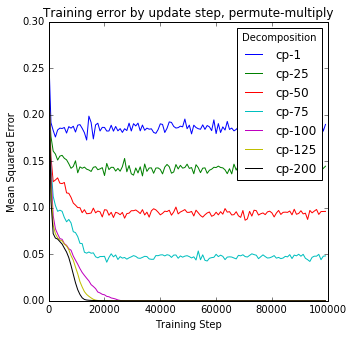
\includegraphics[width=\textwidth]{tensors/permute-cp-mom}
		\caption{Learning curves for CP-decompositions learning permuted 
		element-wise multiplication}
	\end{subfigure}
	~
	\begin{subfigure}[t]{0.45\textwidth}
		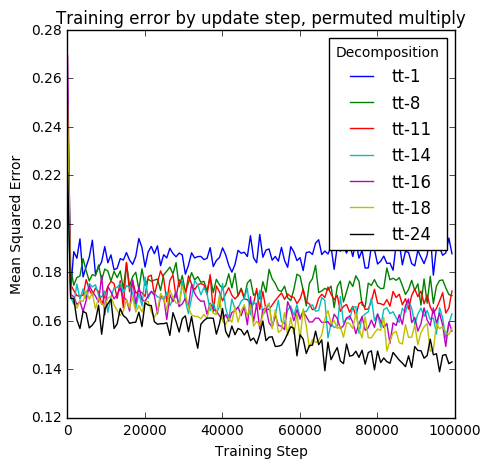
\includegraphics[width=\textwidth]{tensors/permute-tt-mom}
		\caption{Learning curves for TT-decompositions learning permuted
		 element-wise multiplication}
	\end{subfigure}
	\caption{Training error for various rank decompositions on the permuted
	element-wise multiplication
	task.}
	\label{fig:permute-multiply-ff}
\end{figure} 

\section{Synthetic Tasks}
\subsection{Addition}
\subsubsection{Task}
Figure~\ref{fig:additionpics} shows an example input sequence for the addition task discussed in 
section~\ref{sec:addition}. This was generated by training a TGU with 2 hidden units and rank 1
 to solve the
task on sequences of length 50. We show the input to the network and the values of the network's
hidden states.

\begin{figure}
\centering
\begin{tabu} to \textwidth {rX}
states: & 
\includegraphics[width=0.75\textwidth]{exps/addition/states0} \\
inputs: & 
\includegraphics[width=0.75\textwidth]{exps/addition/inputs0}
\end{tabu}

\caption[Addition example]{Example of inputs and states for a network solving the addition task.
Images are greyscale, with lower values darker. The bottom line is the input to the network while the
top row is its hidden states -- clearly it accumulates the appropriate input in a single hidden unit.}
\label{fig:additionpics}
\end{figure}

\subsubsection{Results}
Figure~\ref{fig:addsmall} shows results for the addition task on the smaller of the sequences attempted.
Results are very similar to those at sequence length 750.
\begin{figure}
\centering
\begin{subfigure}[t]{0.75\textwidth}
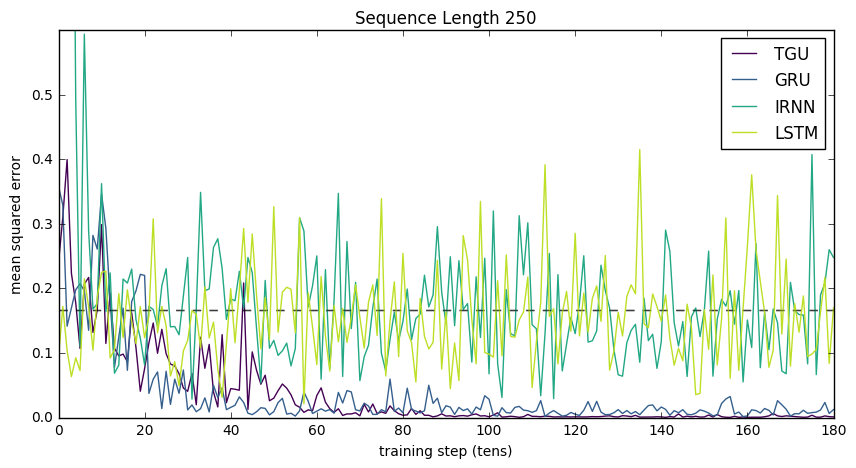
\includegraphics[width=\textwidth]{exps/addition/sl250}
\caption{Sequence length 250.}
\label{fig:add250}
\end{subfigure}

\begin{subfigure}[t]{0.75\textwidth}
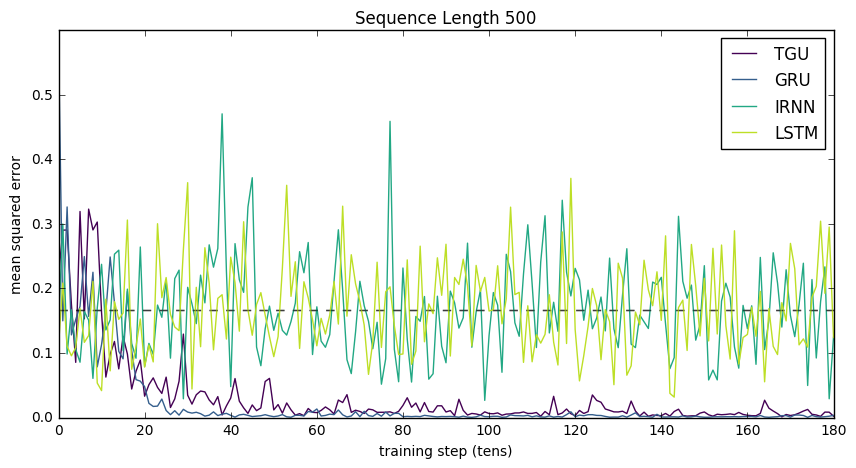
\includegraphics[width=\textwidth]{exps/addition/sl500}
\caption{Sequence length 500.}
\label{fig:add500}
\end{subfigure}
\caption{Addition results, smaller sequences.}
\label{fig:addsmall}
\end{figure}

\subsection{Variable Binding} \label{sec:vbinddata}
\subsubsection{Task}

\begin{figure}
\centering
	\begin{tabu} to \textwidth {XX}
		Input & Target \\
		
\includegraphics[width=0.45\textwidth, interpolate=false]{exps/vbind/100x1input} & 
		
\includegraphics[width=0.45\textwidth, interpolate=false]{exps/vbind/100x1target} \\
		
\includegraphics[width=0.45\textwidth, interpolate=false]{exps/vbind/100x2input} & 
		
\includegraphics[width=0.45\textwidth, interpolate=false]{exps/vbind/100x2target} \\
		
\includegraphics[width=0.45\textwidth, interpolate=false]{exps/vbind/100x3input} & 
		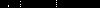
\includegraphics[width=0.45\textwidth, interpolate=false]{exps/vbind/100x3target} \\
	\end{tabu}
	\caption[Example instances of variable binding]{Example input/target pairs for the three
	different variable binding tasks. All have length 100, with 8 bit patterns -- all that differs
	is the number of patterns the network may have to remember at once.}
	\label{fig:vbinddata}
\end{figure}

\begin{figure}
\centering
	\begin{tabu} to \textwidth {XX}
		Input & Output \\
		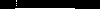
\includegraphics[width=0.45\textwidth, interpolate=false]{exps/vbind/100x1tguinput} & 
		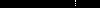
\includegraphics[width=0.45\textwidth, interpolate=false]{exps/vbind/100x1tguoutput} \\
		
\includegraphics[width=0.45\textwidth, interpolate=false]{exps/vbind/100x2tguinput} & 
		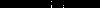
\includegraphics[width=0.45\textwidth, interpolate=false]{exps/vbind/100x2tguoutput} \\
		
\includegraphics[width=0.45\textwidth, interpolate=false]{exps/vbind/100x3tguinput} & 
		
\includegraphics[width=0.45\textwidth, interpolate=false]{exps/vbind/100x3tguoutput} \\
	\end{tabu}
	\caption[Example successful outputs for variable binding]{Outputs from TGU models that that
	achieved good results.}
	\label{fig:vbindcorrect}
\end{figure}

\begin{figure}
\centering
	\begin{tabu} to \textwidth {XX}
		Input & Output \\
		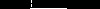
\includegraphics[width=0.45\textwidth, interpolate=false]{exps/vbind/100x1gruinput} & 
		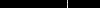
\includegraphics[width=0.45\textwidth, interpolate=false]{exps/vbind/100x1gruoutput} \\
		
\includegraphics[width=0.45\textwidth, interpolate=false]{exps/vbind/100x2gruinput} & 
		
\includegraphics[width=0.45\textwidth, interpolate=false]{exps/vbind/100x2gruoutput} \\
		
\includegraphics[width=0.45\textwidth, interpolate=false]{exps/vbind/100x3gruinput} & 
		
\includegraphics[width=0.45\textwidth, interpolate=false]{exps/vbind/100x3gruoutput} \\
	\end{tabu}
	\caption[Example of baseline for variable binding]{Output from GRUs demonstrating the baseline
	behaviour -- the timing is correct but the output is not related to the input.}
	\label{fig:vbindfail}
\end{figure}

Figures~\ref{fig:vbinddata}, \ref{fig:vbindcorrect} and \ref{fig:vbindfail} all show examples of
the inputs and outputs for the variable binding task. Including the outputs of a successful network
and an network that failed to progress beyond the baseline.

\section{Real Data}

\subsection{Polyphonic Music}
The sizes of the models used are reported in table~\ref{tab:jsbsizes}.


\begin{table}
\begin{tabu} to \linewidth {r||c|c|c|c}
\hline
Model & \multicolumn{4}{|c}{hidden units/rank (parameters)} \\
\hline
Vanilla & \multicolumn{4}{|c}{96  (19927)} \\
LSTM & \multicolumn{4}{|c}{44 (20075)} \\
GRU & \multicolumn{4}{|c}{52 (19763)} \\
\hline
GMR & 95/1 (19870) & 71/35 (19872) & 58/58 (19775) & 45/90 (20125) \\
GMR-C & 349/1 (20005) & 106/52 (20142) & 76/76 (20119) & 53/106 (20248) \\
TGU &  80/1 (20030) & 63/31 (20156) &  53/53 (20248) & 41/82 (19817) \\
TGU-C &  176/1 (20000) & 88/44 (20075) & 66/66 (19855) & 48/96 (20071)\\
\hline
\end{tabu}
\caption[Model sizes for polyphonic music task]{Size of models for polyphonic music
modelling. Architectures with -C appended have the bias matrices combined with the
decomposition. Parameters are reported for inputs of size \(54\) as per the JSB dataset.
Rank is only reported if applicable.}
\label{tab:jsbsizes}
\end{table}

\chapter{Additional Proofs}
There are a number of useful facts which are used throughout the document. Here we provide
proofs of those which are not necessarily obvious.

\section{Element-wise multiplication by bilinear product}
This is a useful point about the structure of a tensor implementing element-wise
multiplication.
\begin{prop} [Identity Tensor] \label{prop:identity}
	\(\tensor{H} \in \mathbb{R}^{N \times N \times N}\) such that
\begin{align}
\vec{x}^\mathsf{T}\tensor{H}\vec{y} = \vec{x} \odot \vec{y}, 
&&\forall \vec{x},\vec{y} \in \mathbb{R}^{N}
\end{align} implies
\begin{equation}
	H_{ijk} = \begin{cases}
		1 & \text{if}\;\;i = j = k \\
		0 & \text{otherwise.}
	\end{cases}
\end{equation}

\end{prop}
\begin{proof}
We prove briefly, by inspecting one component of the result. Let 
\(\vec{z} = \vec{x}^\mathsf{T}\tensor{H}\vec{y}\). Then
\begin{align}
	z_j &= \vec{x}^\mathsf{T}\mat{H}_{\midbullet j \midbullet}\vec{y} \\
		&= \sum_i^N\sum_k^N x_iH_{ijk}y_k
\end{align}
If \(z_j = x_jy_j\) as in the elementwise product, then it is clear we want \(H_{ijk}\) to be 
1 if \(i=j=k\). Further, if we ensure \(H_{ijk}\) is 0 when this is not the case we can see that
the rest of the terms in the sums will disappear.
\end{proof}

\chapter{Initialization}
RNNs can be quite sensitive to initialisation, especially with regard to learning long
time dependencies \autocite{Le2015}. It has been suggested that a good initialisation should
have eigenvalues on or inside the complex unit circle \autocite{Zilly2016, Mikolov2015} which
would suggest initialising to an orthogonal or orthonormal matrix as per \autocite{Henaff2016}.

Figure~\ref{fig:inits} shows some simplified simulation to illustrate the effect of
different methods of initialisation with different forms of gated recurrence. They are
simulated with no non-linearity and a single input at the first time step sampled from a unit
normal. If gate values are required, they are sampled uniformly in \([0,1]\). We then simply
run the recurrence over the hidden state for a number of time steps plotting each cell's state
as a grayscale value.

We show three possible procedures: random normal (mean 0, standard deviation 0.01), spectral
normalised and orthonormal. The spectral normalised matrix is a random normal matrix that
has been divided by a fraction of its leading singular value. This ensures the spectral
radius of the matrix is slightly greater than one. To generate a random orthonormal matrix
we generate a random matrix from a normal distribution, compute its QR decomposition and use the
Q.

\begin{figure}
\centering
\begin{subfigure}[t]{0.3\textwidth}

\includegraphics[width=\textwidth]{appendix/init/vanillanormal}
\caption{Vanilla transition, normal initialisation.}
\end{subfigure}~
\begin{subfigure}[t]{0.3\textwidth}

\includegraphics[width=\textwidth]{appendix/init/lstmnormal}
\caption{Forget gate transition, normal initialisation.}
\end{subfigure}~
\begin{subfigure}[t]{0.3\textwidth}

\includegraphics[width=\textwidth]{appendix/init/grunormal}
\caption{Convex gate transition, normal initialisation.}
\end{subfigure}\\

\begin{subfigure}[t]{0.3\textwidth}

\includegraphics[width=\textwidth]{appendix/init/vanillaspec}
\caption{Vanilla transition, spectral normalised initialisation.}
\end{subfigure}~
\begin{subfigure}[t]{0.3\textwidth}

\includegraphics[width=\textwidth]{appendix/init/lstmspec}
\caption{Forget gate transition, spectral normalised initialisation.}
\end{subfigure}~
\begin{subfigure}[t]{0.3\textwidth}
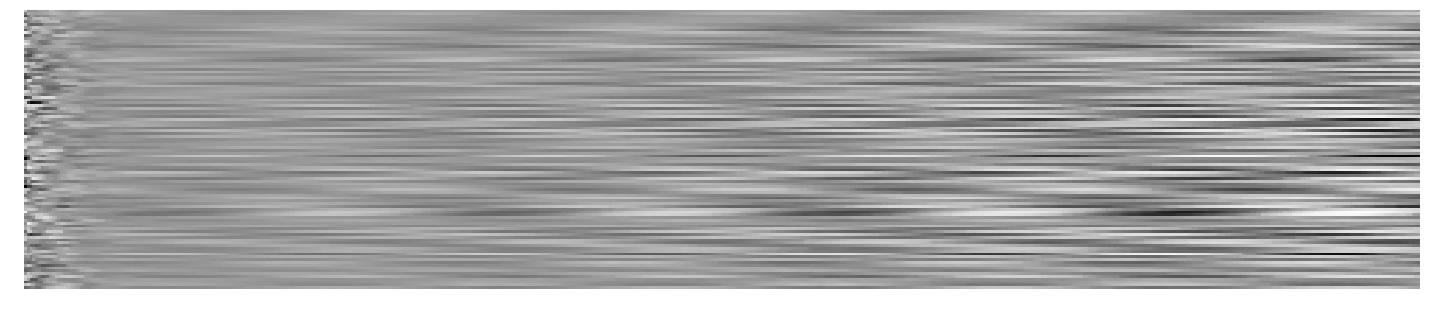
\includegraphics[width=\textwidth]{appendix/init/gruspec}
\caption{Convex gate transition, spectral normalised initialisation.}
\end{subfigure}\\

\begin{subfigure}[t]{0.3\textwidth}

\includegraphics[width=\textwidth]{appendix/init/vanillaorth}
\caption{Vanilla transition, orthonormal initialisation.}
\end{subfigure}~
\begin{subfigure}[t]{0.3\textwidth}

\includegraphics[width=\textwidth]{appendix/init/lstmorth}
\caption{Forget gate transition, orthonormal initialisation.}
\end{subfigure}~
\begin{subfigure}[t]{0.3\textwidth}
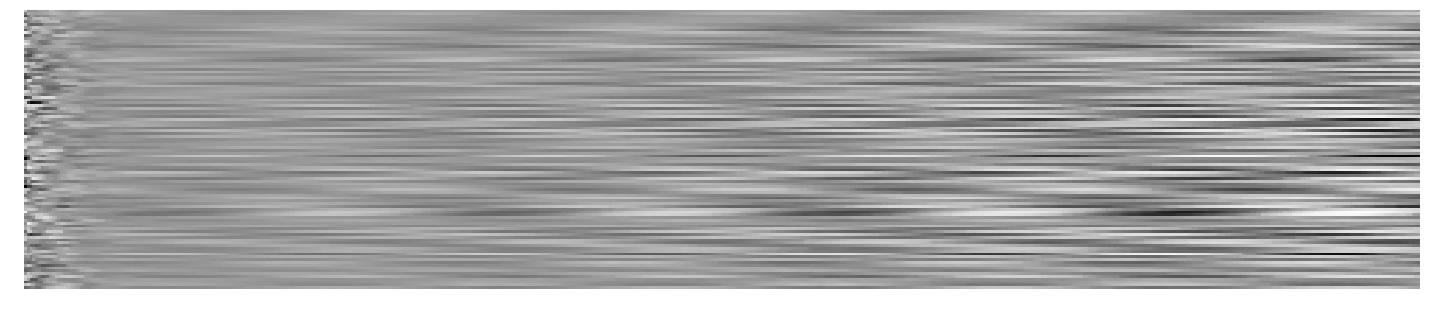
\includegraphics[width=\textwidth]{appendix/init/gruspec}
\caption{Convex gate transition, orthonormal initialisation.}
\end{subfigure}\\

\caption{Example simulations of RNN states from different initialisation. Images are
independently normalised, with darker values being more negative and lighter more positive.}
\label{fig:inits}
\end{figure}

Results are in figure~\ref{fig:inits}. Clearly initialising from a normal distribution is
insufficient. The spectral normalisation also tends to explode (note that often the initial
random state is no longer visible, this is because the degree of normalisation required
to display the final states). Correspondingly we prefer the orthonormal initialisation
throughout this report, although we note that with Vanilla RNNs which preserve information
nearly perfectly from this initialisation we occasionally had to scale the entire matrix down
by a constant factor to avoid exploding early in training.


\chapter{Algorithms for Synthetic Tasks}

\section{Addition}\label{sec:additionpseudo}
Data for the addition task can be generated by algorithm~\ref{alg:additiondata}. This algorithm
produces a single item, it could also be done in batches with slight adjustments.

\begin{algorithm}
	\KwIn{Integer \(T\)}
	\KwOut{Problem instance \((\vec{x}_1, \vec{x}_2, \ldots, \vec{x}_T), y\)}
	\BlankLine
	Sample integer \(i \sim U[1, (T/2)-1]\)\;
	Sample integer \(j \sim U[T/2, T]\)\;
	\(y \gets 0\)\;
	\For{\(t \in \{1, \ldots, T\}\)}{
		Sample float \(x_{t1} \sim U[0,1]\)\;
		\If{\(t = i\) or \(t = j\)} {
			\(y \gets y + x_{t1}\)\;
			\(x_{t2} \gets 1\)\;
		} \Else {
			\(x_{t2} \gets 0\)\;
		}
	}
	\KwRet{\((\vec{x}_1, \vec{x}_2, \ldots, \vec{x}_T), y\)}
	\caption{Generating data for addition task}
	\label{alg:additiondata}
\end{algorithm}

\section{Variable binding}\label{sec:vbindpseudo}
Algorithm~\ref{alg:vbinddata} shows how to generate a single data item for this task. This algorithm
is indicative only, there are ways to be more efficient especially if it has to be implemented as a
computation graph, for example in Tensorflow.

\begin{algorithm}
	\KwIn{Integers \(T, D, N\)}
	\KwOut{Problem instance \((\vec{x}_1,\ldots,\vec{x}_T), (\vec{y}_1,\ldots,\vec{y}_T)\)}
	\BlankLine
	intialise \((\vec{x}_1,\ldots,\vec{x}_T), (\vec{y}_1,\ldots,\vec{y}_T)\) to zeros\;
	\For{\(i \in \{1, \ldots, N\}\)} {
		Sample integer \(j \sim U[1, (T/2)-1]\) \tcc*{start position}
		Sample integer \(k \sim U[j+1, T]\) \tcc*{end position}
		\(\vec{z} \gets\) random \(D\) bit binary pattern\;
		\(\vec{y}_{k+1} \gets \vec{z}\)\;
		Set first \(D\) bits of \(\vec{x}_{i+1}\) to \(\vec{z}\)\;
		\For(set label bits){\(l \in \{j,\ldots,k\}\)}{
			\({x}_{l, D+i} \gets 1\)\;
		}
	}
	\KwRet{\((\vec{x}_1,\ldots,\vec{x}_T), (\vec{y}_1,\ldots,\vec{y}_T)\)}
	
	\caption{Generating data for variable binding}
	\label{alg:vbinddata}
\end{algorithm}